\NeedsTeXFormat{LaTeX2e}
%\PassOptionsToClass{handout}{beamer}
\documentclass{beamer}
\usepackage{beamerPack}
\usepackage[boxed,ruled,vlined]{algorithm2e}
\usepackage{bm}
\usepackage[01]{../lecture}
\subtitle{探索}
\begin{document}

\begin{frame}[fragile]{}
\titlepage
\end{frame}

\section{Intro}		%%%%%%%%
\subsection{}

\begin{frame}[fragile]{アウトライン}{}
トピックス
\begin{itemize}
\item 代表的な探索アルゴリズム
\item 計算量の理論
\item 代表的な整列アルゴリズム
\item 共通要素の抽出
\item 動的計画法
\end{itemize}

\vfill
参考文献
\begin{itemize}
\item Wikipedia
\item Donald E. Knuth: The Art of Computer Programming
\end{itemize}
\end{frame}

\begin{frame}[fragile]{設定}{}

\begin{exampleblock}{ハードウェア}
\begin{itemize}%\itemsep8pt
\item 単一CPU
\item メモリのアクセス速度一定
\item 機械語を実行
\end{itemize}
\end{exampleblock}

\begin{exampleblock}{プログラミング言語}
\begin{itemize}%\itemsep8pt
\item 配列型{\tt Vec<T>}を有する
\begin{itemize}%\itemsep8pt
\item 添字は0から始まる自然数(最終要素の添字は長さ-1)
\item アクセス速度一定
\end{itemize}
\item 関数が定義できる、再帰呼出しできる
\item 実行前に機械語に変換
\end{itemize}
\end{exampleblock}
\end{frame}

\section{Search}		%%%%%%%%
\subsection{}

\begin{frame}[fragile]{探索}{メモリに置かれたデータの中からある条件を満たす要素があるかどうかを判定}
$\to$配列の中からある条件を満たす要素の存在を判定

\footnotetext[1]{二分検索: 2,550, 二分探索:89,800}

\vfill
\begin{center}
\scalebox{0.6}{
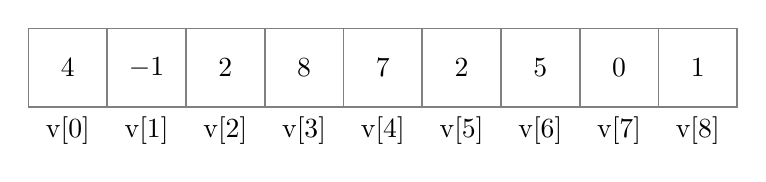
\begin{tikzpicture}[
    , cell/.style = {rectangle,draw=gray,semithick,minimum size=1cm,outer sep = 0mm,label=below:v{[\j]}}
]
\foreach \i [count=\j from 0] in {4, -1, 2, 8, 7, 2, 5, 0, 1}
    \node[cell] at (\j, 0) {$\i$};
\end{tikzpicture}
}
\end{center}

\vfill
\begin{codeof}{language=Rust}{ライブラリより(自動並列化や逆順走査の可能性)}
  x = v.find(...);             // ライブラリ関数find
  if v.iter().any(|x| c(x)) {  // どれかがtrueになればtrue
\end{codeof}
\end{frame}

\section{Linear search}		%%%%%%%%
\subsection{}

\begin{frame}[fragile]{探索アルゴリズム1:一つずつ調べる}{}
\scalebox{0.9}{
\begin{algorithm}[H]
\KwIn{v: \texttt{Vec<T>}}
\KwIn{条件 --- 引数を二分判定する関数}
\KwOut{発見または失敗}
\SetKwComment{Comment}{}{}
\BlankLine
i = 0\Comment*{\sl\small\color[gray]{0.5} 添字を表すローカル変数}
\While{iが要素数より小さい} {
  \If{v[i]が条件を満たす}{
    \Return{発見}
  }
  i += 1\;
}
\Return{失敗}\;
\caption[page]{線形探索}
\end{algorithm}
}
\vfill
アルゴリズムから見える構造
\begin{itemize}%\itemsep8pt
\item 1ステップごとに残りが減っていく: $[0, N) \to [1, N) \to \cdots$
\item 1ステップごとに(範囲を変えて)同じ処理
\end{itemize}
\end{frame}

\begin{frame}[fragile]{TypeScriptで実装}{\href{https://replit.com/@shnarazk/LinearSearchInTypeScript}{\beamergotobutton{replit.com/@shnarazk/LinearSearchInTypeScript}}}
\begin{codeof}{language=C}{lsearch}
function lsearch<T> (v: Array<T>, c: (e:T) => boolean): boolean {
  let i = 0
  while (i < v.length) {
    if (c(v[i])) { return true }
    i += 1

const vec = [1, 4, 8, 9, -1, -2, 8, 10]

// test case 1
function equal_8 (i: number): boolean { return i === 8 }
console.log(lsearch(vec, equal_8))
\end{codeof}
\end{frame}

\begin{frame}[fragile]{チェックリスト}{}

\begin{enumerate}\itemsep20pt
\item アイテム指定(例えば3)だけでなく、条件指定(例えば偶数)もできること
\item 特定の型(例えばnumber)だけでなく、別の型(例えばstring)にも適用できること
\item 探索目的が場所(添字)の報告なら、大きな変更なく対応できること
\end{enumerate}
\end{frame}

\begin{frame}[fragile]{アルゴリズムの評価尺度}{}

\begin{itemize}%\itemsep8pt
\item 停止性\href{https://ja.wikipedia.org/wiki/アルゴリズム}{\beamergotobutton{アルゴリズムの定義について}}
\item 正確さ(完全性)-- 間違える可能性
\item 適用範囲\footnotemark
\item 速度
\end{itemize}
\vfill
本来はアルゴリズムの段階で考えるべき

{\fontsize{8}{9}\selectfont
\begin{tabular}[h]{|p{0.12\textwidth}|p{0.6\textwidth}}
\CH 尺度 & 線形探索 \\\hline
\CL 停止性 & 配列長さが繰り返し上限になっているので問題ない \\
\CL 完全性 & 全ての要素を調べているので問題ない \\
\CL 適用対象 & 同一性判定できること  \\
\CL 速度 & 説得力のある定義が必要  \\
\end{tabular}
}
\vfill
利用可能かどうかを考慮した後に速度
\footnotetext[1]{要素の型Tに課せられた制約}
\end{frame}

\begin{frame}[fragile]{Rustで実装}{\href{https://replit.com/@shnarazk/LinearSearchInRust\#src/lsearch.rs}{\beamergotobutton{replit.com/@shnarazk/LinearSearchInRust\#src/lsearch.rs}}}
\begin{codeof}{language=Rust}{lsearch (lsearch.rs)}
/// `v: [T]`に対して条件`c`を満たす要素を線形探索し、...
/// ```
/// use crate::toa::lsearch::lsearch;
///
/// let vec: Vec<i32> = vec![1, 4, 8, 9, -1, -2, 8, 10];
/// assert_eq!(lsearch(&vec, |i| *i == 8i32), true);
/// ```
fn lsearch<T>(v: &[T], c: impl Fn(&T) -> bool) -> bool {
    let mut i = 0;
    while i < v.len() {
        if c(&v[i]) { return true; }
        i += 1;
    }
    false
}
\end{codeof}
\end{frame}

\section{Binary search}		%%%%%%%%
\subsection{}


\begin{frame}[fragile]{別の探索アルゴリズム}{}
線形探索は探索範囲を調査済みとそうでない部分に分割し、1ステップにつき1つずつ探索範囲を縮小
\vfill
1ステップで複数個縮小できないか
\vfill
ある範囲に対して代表する要素を与え、それを調べることでその範囲を全て調べたことにできればよい

\begin{center}
\scalebox{0.6}{
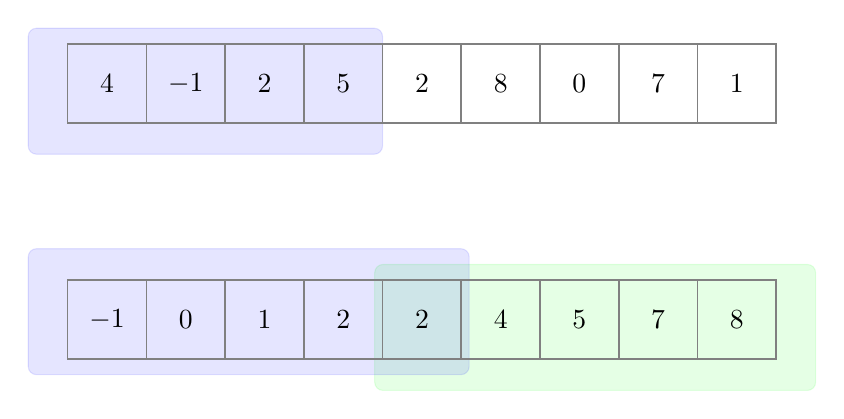
\begin{tikzpicture}[
    , cell/.style = {rectangle,draw=gray,semithick,minimum size=1cm,outer sep = 0mm}
]
\draw[draw=blue,fill=blue,rounded corners=3,anchor=west,opacity=0.1] (-1,2.1) rectangle ++(4.5,1.6) {};
\draw[draw=green,fill=green,rounded corners=3,anchor=west,opacity=0.1] (3.4,-0.9) rectangle ++(5.6,1.6) {};
\draw[draw=blue,fill=blue,rounded corners=3,anchor=west,opacity=0.1] (-1,-0.7) rectangle ++(5.6,1.6) {};
\foreach \i [count=\j from 0] in {4, -1, 2, 5, 2, 8, 0, 7, 1}
    \node[cell] at (\j, 3) {$\i$};
\foreach \i [count=\j from 0] in {-1, 0, 1, 2, 2, 4, 5, 7, 8}
    \node[cell] at (\j, 0) {$\i$};
\end{tikzpicture}
}
\end{center}
\end{frame}

\begin{frame}[fragile]{探索アルゴリズム2: 探索範囲を半分}{}
\scalebox{0.9}{
\begin{algorithm}[H]
\KwIn{v: \texttt{Vec<T>} ---(前提条件)要素は小さい順に整列ずみ}
\KwIn{条件 --- 要素を小さい、等しい、大きいに三分判定}
\KwOut{発見または失敗}
\SetKwComment{Comment}{}{}
\BlankLine
i = 0\Comment*{\sl\small\color[gray]{0.5}探索範囲の左の添字}
j = z.len() - 1\Comment*{\sl\small\color[gray]{0.5}探索範囲の右の添字}
\While{i <= j} {
  \If{ v[(i + j) / 2]の判断結果が「等しい」}{
    \Return{発見}
  }
  \eIf{v[(i + j) / 2]の判断結果が「小さい」}{
    i = (i + j) / 2 + 1\Comment*{\sl\small\color[gray]{0.5}探索範囲の左半分を破棄}
  }{
    j = (i + j) / 2 - 1\Comment*{\sl\small\color[gray]{0.5}探索範囲の右半分を破棄}
  }
}
\Return{失敗}\Comment*{\sl\small\color[gray]{0.5}なお整数割算の結果は整数を仮定}
\caption[page]{二分探索}
\end{algorithm}
}
\end{frame}

\begin{frame}[fragile]{二分探索のTypeScriptによる実装}{\href{https://replit.com/@shnarazk/BinarySearchInTypeScript}{\beamergotobutton{replit.com/@shnarazk/BinarySearchInTypeScript}}}
\begin{codeof}{language=C}{bsearch (index.ts)}
type Ord = -1 | 0 | 1 // 小さい/等しい/大きい、に対応

function bsearch<T>(v:Array<T>, c:(e:T) => Ord): boolean {
  let i: number = 0
  let j: number  = v.length - 1
  while (i <= j) {
    const mid = Math.floor((i + j) / 2)  // 明示的な整数化
    switch (c(v[mid])) {
      case -1: j = mid - 1; break;       // 左半分に行く
      case  0: return true;
      case  1: i = mid + 1; break;       // 右半分に行く
    }
  }
  return false
}

function cond (e: number): Ord { return Math.sign(8-e) }
\end{codeof}
\end{frame}

\begin{frame}[fragile]{二分探索のRustによる実装}{\href{https://replit.com/@shnarazk/LinearSearchInRust\#src/bsearch.rs}{\beamergotobutton{replit.com/@shnarazk/LinearSearchInRust\#src/bsearch.rs}}}
\begin{codeof}{language=C}{bsearch (bsearch.rs)}
use std::cmp::Ordering;
/// ```
/// use crate::toa::bsearch::bsearch;
/// let vec: Vec<i32> = vec![-2, -1, 1, 4, 8, 8, 9, 10];
/// assert_eq!(bsearch(&vec, |i| 8i32.cmp(i)), true);
/// ```
pub fn bsearch<T>(v: &[T], c: impl Fn(&T) -> Ordering) -> bool {
    let (mut i, mut j) = (0,  v.len() - 1);
    while i < j {
        let mid = (i + j) / 2;
        match c(&v[mid]) {
            Ordering::Less => j = mid - 1,
            Ordering::Equal => return true,
            Ordering::Greater => i = mid + 1,
        }
    }
    false
}
\end{codeof}
\end{frame}

\begin{frame}[fragile]{検討}{}

{\fontsize{8}{9}\selectfont
\begin{tabular}[h]{|p{0.12\textwidth}|p{0.4\textwidth}|p{0.4\textwidth}|}
\CH 尺度 & 線形探索 & 二分探索 \\
\CL 停止性 & 配列長さが繰り返し上限 & 探索範囲$j - i$は単調減少\footnotemark、かつ0で終了 \\
\CL 完全性 & 全ての要素を調べているので問題ない & 前提条件より導出可能 \\
\CL 適用対象 & 同一性判定できること & 全順序であること、かつ配列が整列ずみ \\
\CL 速度 & 遅そうだが説得力のある定義が必要 & 速そうだが説得力のある定義が必要\\
\end{tabular}
}

\vfill
条件のバリエーション「最大値の探索」:
条件が要素間の関係上に定義されるものだからこのフレームワークでは無理

\footnotetext[1]{iは単調増加、jは単調減少}
\end{frame}

\section{Appendix}		%%%%%%%%
\subsection{}

\begin{frame}[fragile]{その他の探索}{}
\begin{itemize}\itemsep20pt%[<+->]
\item ハッシュ表
\begin{itemize}%\itemsep8pt
\item 特定の探索条件に対して二分探索より高速
\item 正確にはハッシュ表というデータ構造{\footnotemark}とハッシュ関数のペア
\item 速度の点では有利だが別の観点で不利
\item Python: Dictionary, JavaScript: Object
\end{itemize}
\item データ分布の偏りを利用するもの
\item 設定の違い:木探索、グラフ探索、ヒューリスティックスなど
\end{itemize}
\footnotetext[1]{配列で実現可能}
\end{frame}

\end{document}
